\section{Forward and backward propagation}

  Following the definitions in Section~\ref{sec-conv-layers}, the
  forward propagation algorithm can be used for the backward
  propagation if we (1) reflect the kernels, thus converting
  convolution to cross--correlation, and (2) zero--pad the input image
  such that \texttt{valid} cross--correlation becomes \texttt{full}
  cross--correlation.

  We propose an algorithm for the forward propagation that can handle
  implicit zero--padding of the input images.  Hence, the same
  algorithm can be used for the backward propagation with no overhead.
  As previously stated, we assume that two copies of kernels are
  stored and maintained in memory - original and reflected.  This is
  reasonable because the memory required for kernels is typically much
  smaller than the memory required for the images.

  We will refer to the algorithm as the \emph{propagation algorithm}.
  Also, we'll refer to both the input/output images of the forward
  propagation ($I$ and $I'$) and the output/input gradients of the
  backward propagation ($\hat{I}$ and $\hat{I}'$) as simply
  \emph{input/output images}.

  \subsection{Algorithm overview}

  The further discussion assumes that both $F$ and $F'$ are divisible
  by $S$ ($F = \alpha S$ and $F' = \alpha' S$.  Nearly all state of
  the art ConvNets for both registration and segmentation have both
  $F$ and $F'$ being a large multiple of
  $2$~\cite{krizhevsky2012imagenet, ronneberger2015u,
    simonyan2014very, sermanet2013overfeat, long2015fully,
    tran2015learning, ji20133d, maturana_iros_2015,
    maturana_icra_2014}.  An arbitrary number of images can be
  implemented by simply adding zero--initialized dummy images.  As
  both $F$ and $F'$ are relatively large, this would not introduce
  much computational overhead.  In our public repository, however, we
  also provide the implementation for this specific cases that has no
  overhead.

  Our algorithm consists of a stack of primitives with increasing
  complexity.  Each more complex primitives uses the less complex ones
  to perform more complex computation.  We list the primitives in the
  increasing order of complexity together with the main motivation and
  goal for each one.

  \begin{enumerate}
  \item {\bf Sub--image primitive} computes $S^2$ convolutions on $S$
    small images producing $S$ small images of size $R_x, R_y, R_z$.
    The goal of this primitive is to efficiently re--use data in the
    register file as well as data in L1 cache.  The technique used by
    the primitive is known as register blocking.
  \item {\bf Full image primitive} computes $S^2$ convolutions on $S$
    input images of an arbitrary size, producing $S$ output images.
    The primitives optimally divides the computation into small blocks
    for which the previous primitive is used.  The division and order
    of computation is designed for efficient use of hardware
    pre--fetching and higher cache levels.
  \item {\bf Sub--layer primitive} computes $\beta S$ images by
    performing $\alpha \beta S^2$ convolutions on $\alpha S$ images.
    The primitive is designed to efficiently utilize higher cache
    levels.
  \item {\bf Full layer primitive} divides the computation into
    sub--layer primitives and statically schedules their execution on
    the available cores.  The goal is to evenly divide the computation
    among available cores.
  \end{enumerate}

  \begin{algorithm}
    {\footnotesize
      \begin{codebox}
        \Procname{$\proc{Fwd-Bwd-Subtask} \langle \Theta, R_x, R_y, R_x, K_x, K_y, K_z \rangle(i,w,i',\theta)$}
        \li \kw{simd float} $oreg[R_x][R_y][R_z]$
        \li \kw{simd float} $wreg$
        \li \If $\Theta$ \Comment Static if
        \li \Then $oreg[:][:][:][:] \gets \theta$ \Comment Load bias
        \li \Else
        \li       $oreg[:][:][:][:] \gets \proc{LOAD}(i'[:][:][:][:])$
        \End \li \kw{end if}
        \li \kw{for} $k_x \gets 0 \To K_x-1$ \Comment Partially unrolled
        \li   \Do \kw{for} $k_y \gets 0 \To K_y-1$  \Comment Partially unrolled
        \li     \Do \kw{for} $f \gets 0 \To S - 1$ \Comment Partially unrolled
        \li       \Do \kw{for} $k_z \gets 0 \To K_z-1$  \Comment Conditionally unrolled
        \li         \Do $wreg \gets w[k_x][k_y][k_z][f][:]$
        \li \kw{for} $x \gets 0 \To R_x-1$ \Comment Fully unrolled
        \li   \Do \kw{for} $y \gets 0 \To R_y-1$ \Comment Fully unrolled
        \li      \Do \kw{for} $z \gets 0 \To R_z-1$ \Comment Fully unrolled
        \li         \Do $oreg[x][y][z][:] \gets \proc{FMADD}($
        \li       $wreg,$
        \li       $\proc{EXLOAD}(i[x+k_x][y+k_y][z+k_z][f]),$
        \li       $oreg[x][y][z][:])$
        \End \li \kw{end for} $z$
        \End \li \kw{end for} $y$
        \End \li \kw{end for} $x$
        \End \li \kw{end for} $k_z$
        \End \li \kw{end for} $f$
        \End \li \kw{end for} $k_y$
        \End \li \kw{end for} $k_x$
        \li $i'[:][:][:][:] \gets \proc{STORE}(oreg[:][:][:][:])$
      \end{codebox}
    \caption{The finest granularity primitive that computes a
      sub--image of size $R_x \times R_y \times R_z$ of $S$ images by
      performing $S^2$ cross--correlations on $S$ input images with
      kernels of size $K_x \times K_y \times K_z$.}
    \label{alg:serial-forward-subtask}
    }
  \end{algorithm}

  {\bf Sub--image primitive} is shown in
  Algorithm~\ref{alg:serial-forward-subtask}.  The arguments inside
  the angle brackets are known during compile--time.  (This is easily
  implemented using C++ templates).  The arguments are mostly loop
  bounds, which enable the compiler to perform loop unrolling as
  commented in the pseudo--code.  Another argument $\Theta$ specifies
  whether the result of the cross--correlation will be accumulated to
  an existing image $i'$, or to a bias $\theta$.

  Taking into account the data layout and Equation~\ref{eq:forward},
  each value of the memory array $i'[r_x][r_y][r_z][f']$ is computed
  via {\footnotesize
  \[
  \sum_{f} \sum_{k_x} \sum_{k_y} \sum_{k_z}
  i[r_x+k_x][r_y+k_y][r_z+k_z][f] \cdot w[k_x][k_y][k_z][f][f']
  \]
  } Our data layout allows for natural vectorization over $f'$.  $S$
  results $i'[r_x][r_y][r_z][:]$ are computed by replacing the scalar
  product to a scalar--vector product {\footnotesize
  \[
  \sum_{f} \sum_{k_x} \sum_{k_y} \sum_{k_z}
  i[r_x+k_x][r_y+k_y][r_z+k_z][f] \cdot w[k_x][k_y][k_z][f][:]
  \]
  }
  We recognize that the values $w[k_x][k_y][k_z][f][:]$ are used for
  computing all $i'[r_x][r_y][r_z][:]$ and reorder the computation
  such that once $w[k_x][k_y][k_z][:]$ is loaded (line 12) from
  memory, it is maximally re--used.
  
  In the multiply--add operation of lines 16--19, the procedure
  $\proc{EXLOAD}$ loads a scalar value to all $S$ locations in a
  vector register.  The CPU-dependent macro $\proc{FMADD}$ either
  calls the fused multiply--add intrinsic (AVX2), or vector
  multiplication followed by a vector addition (AVX, SSE4).  AVX512
  supports a single instruction that performs fused multiply--add with
  the multiplication performed by an in--memory scalar.

  Iterating the three innermost loops (lines 13-15) yields $R_x \times
  R_y \times R_z$ independent multiply-add operations.  This number
  should be large to maximize utilization. At the same time, $oreg$,
  $wreg$ and all possible auxiliary variables should fit into the
  register file.  For AVX512, $wreg$ takes one vector register leaving
  31 others for $oreg$, so the maximal limit for $R_x \times R_y
  \times R_z$ is 31.  SSE4, AVX, and AVX2 require auxiliary registers
  for loading the scalar value, so choosing the maximal limit requires
  a bit more analysis.

  Note how the loop over $f$ comes before the loop over $k_z$.  As
  $k_z \ge 2$ in convolutional layers, we expect the compiler to
  unroll the loop over $k_z$.  When auxiliary registers are required,
  the compiler is expected to reorder the load and multiply--add
  operations such that the values loaded in the auxiliary registers
  are re--used.  As discussed above, to fully utilize the CPU we need
  to issue $nl$ (number of FMA units times the instruction latency)
  independent consecutive instructions.  As each auxiliary register is
  re--used approximately $k_z$ times, we need $nl/k_z$ auxiliary
  registers to fully saturate the vector units.  As $k_z \ge 2$ we
  choose to use $10$ registers for $oreg$, allowing for $5$ auxiliary
  registers.  This choice allows for saturating CPUs for which $nl \le
  8$ which is true for all modern CPUs.

  The working set of the primitive is expected to fit inside the $L1$
  cache.  This is a reasonable expectation as the size of $R_x \times
  R_y \times R_z$ is very limited, and the kernel sizes are expected
  to be small.  The cache miss rate can be thus approximated to
  $\frac{1}{C \times K_x \times K_y \times K_z}$, where $C$ is the
  number of floats that fit inside the cache--line (typically $C$ =
  16).  This value is very low for even tiny kernels.  The regular
  memory access pattern (linear along $z$ dimension) allows for
  further reduction in cache misses due to hardware pre--fetching.
  Measured cache hits averaged to over $98\%$ of kernel sizes of $1
  \times 2 \times 2$ or larger, and any appropriate size of $R_x
  \times R_y \times R_z$.

  \begin{figure}
    \begin{center}
      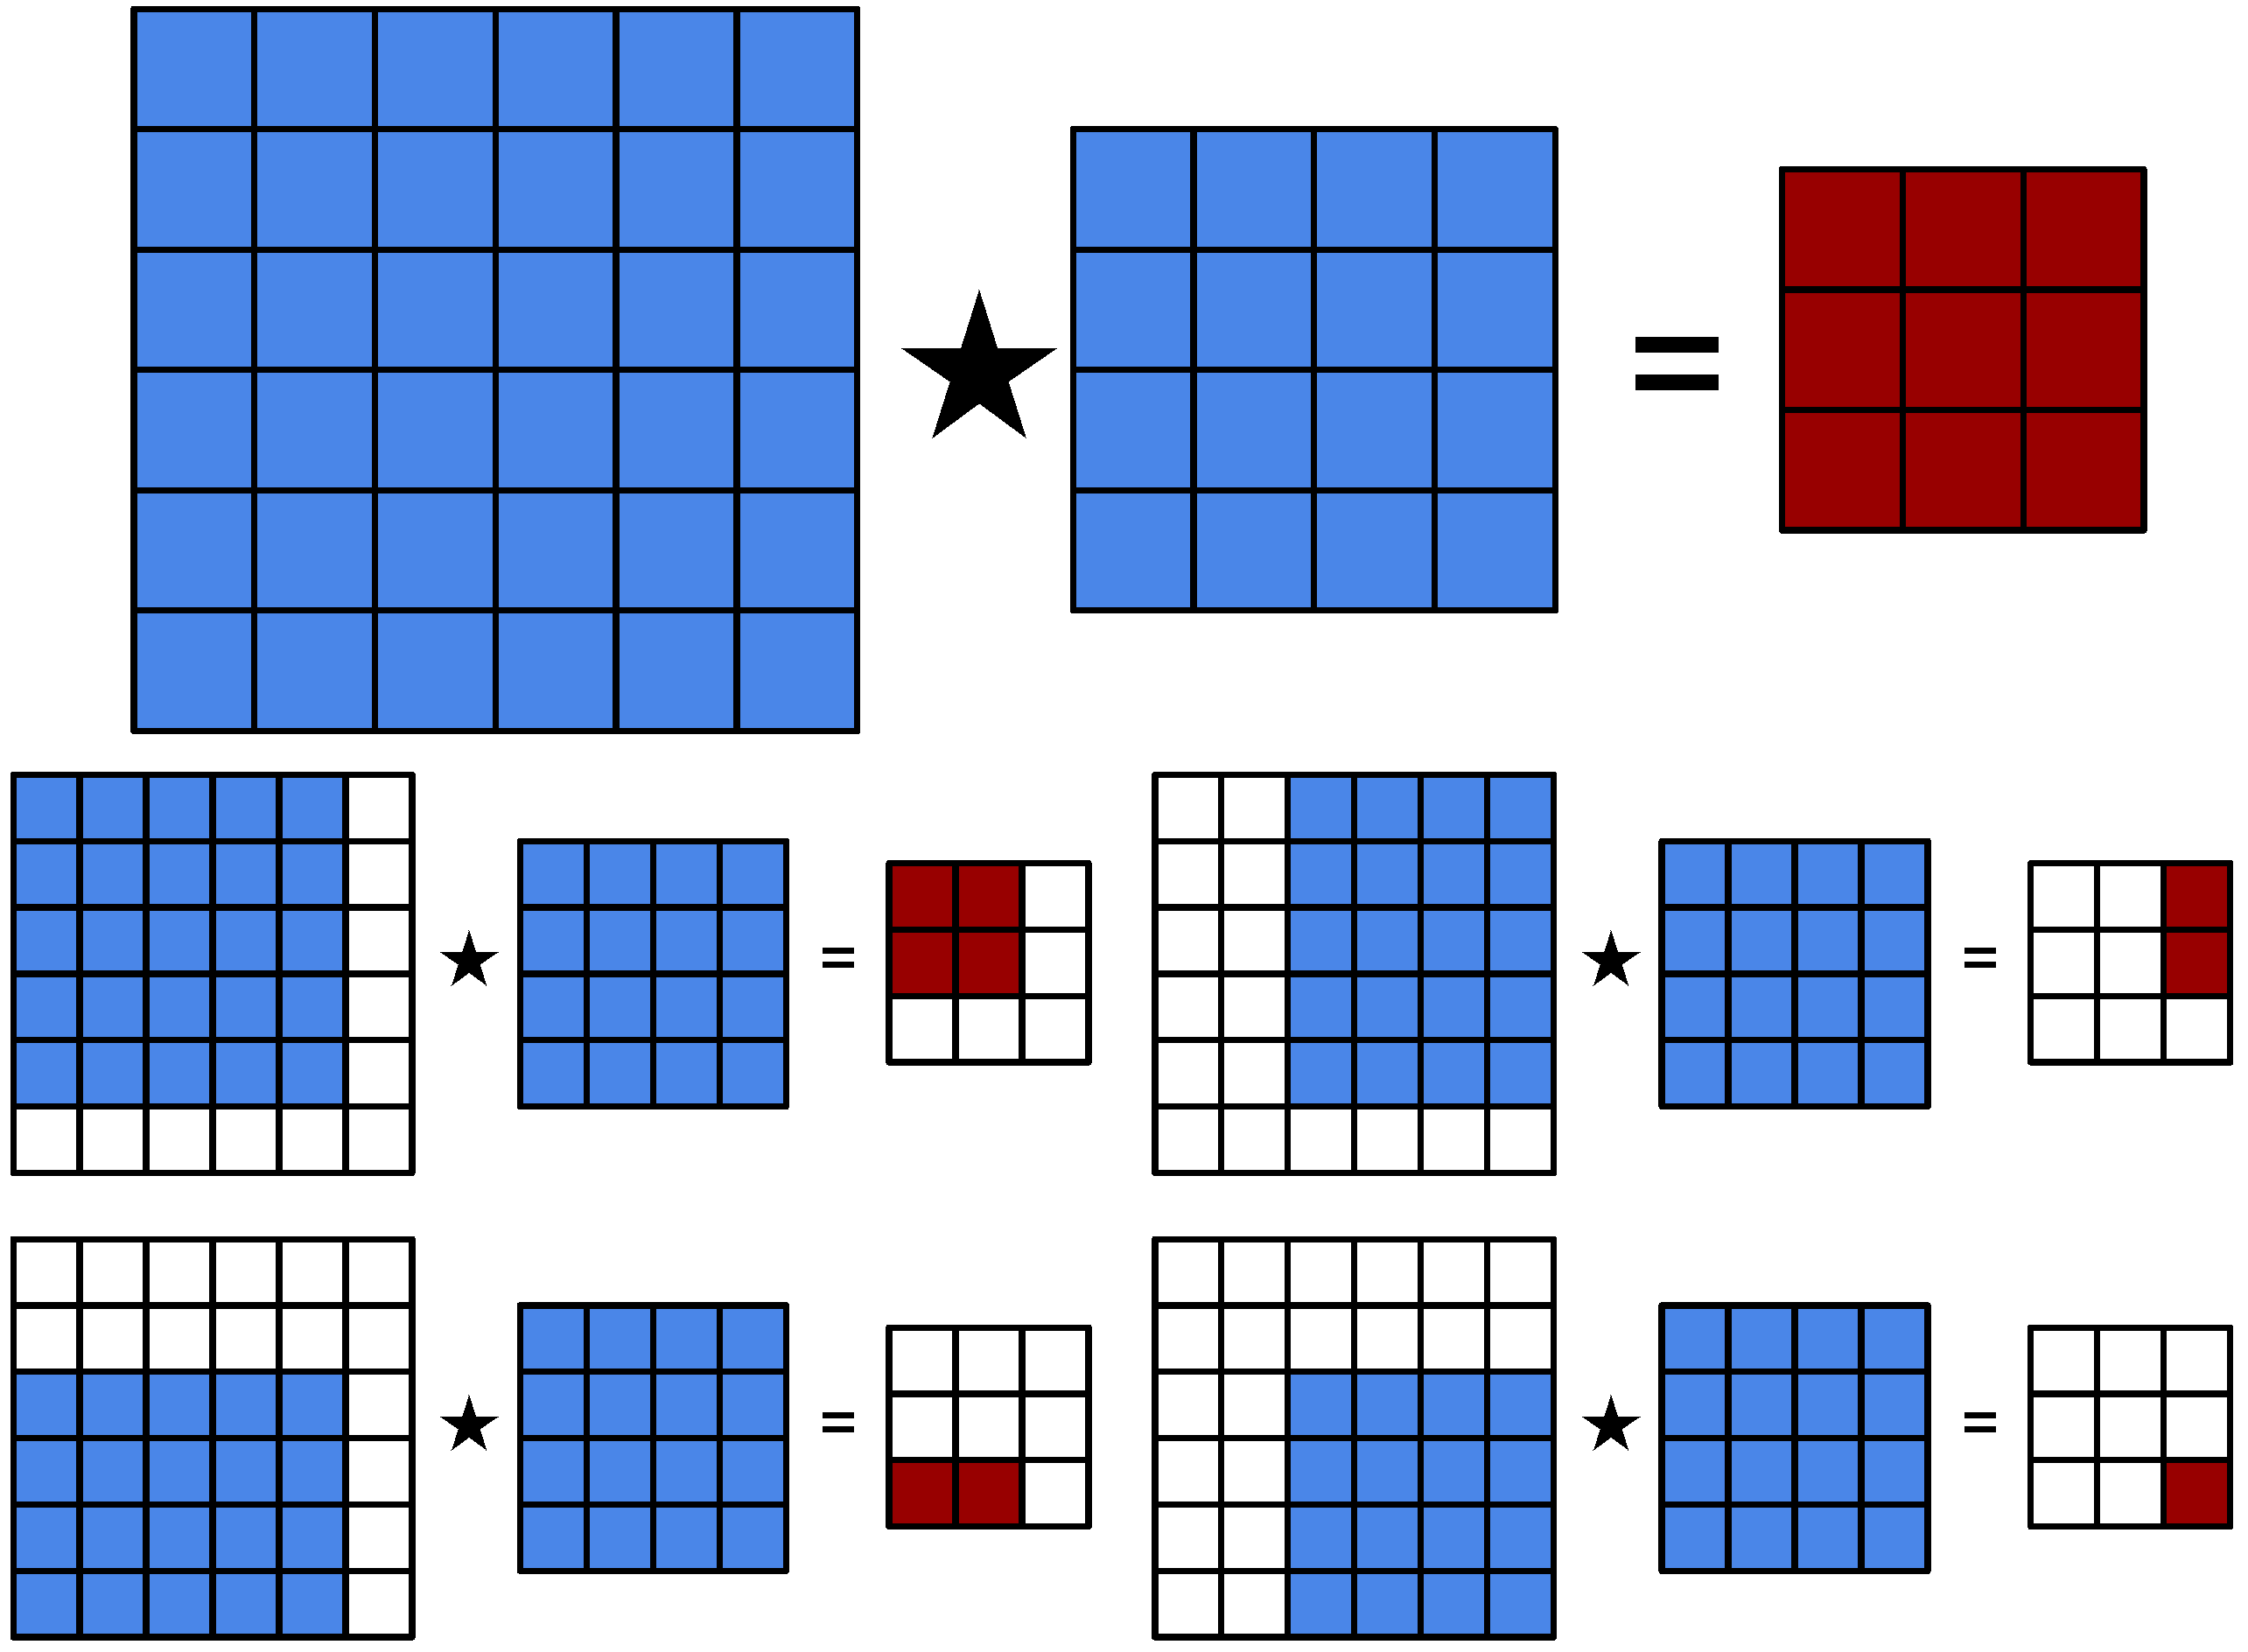
\includegraphics[width=0.57\linewidth]{fig/division}
    \end{center}
    \caption{Computing sub--results of cross--correlation as
      cross--correlation of sub--images.}
    \label{fig:conv-division}
  \end{figure}

  {\bf Full image primitive} performs $S^2$ cross--correlations on $S$ images
  of an arbitrary size, producing $S$ output images of size $N_x'
  \times N_y' \times N_z'$.  This is done by dividing the output
  images into small sub--images (Fig~\ref{fig:conv-division} and using
  the primitive described above.  The size of each sub--image should
  be maximized, but is subject to constraints described above.  We
  prefer division into sub--images with large values of the least
  significant dimension, such that the adjacent pixels are adjacent in
  memory, thus benefit from hardware pre--fetching.  As the image
  dimensions are typically larger than $R$ (number of registers
  available for $oreg$, as described above), in most case, the image
  will be split into sub--images of size $1 \times 1 \times R$.
  Alternatively, we will try the subdivision into $1 \times 2 \times
  \floor{R/2}$, etc...  Note that in most cases we will not be able to
  subdivide the image into equal parts.  This is handled by
  instantiating separate primitives for different sub--image sizes.
  This will result in the image fully covered in tiles, not all of
  which will have the same size.  However, we will have an optimally
  compiled code for each of them.

  The computation is then performed tile by tile, sliding along the
  least significant direction first, then the second least
  significant, etc...  This order of computation has multiple
  benefits.  First, it can benefit from hardware pre--fetching.
  Secondly, accessing contiguous data minimizes possible cache
  associativity conflicts, allowing us to store more data in the
  higher levels of cache.  This values can be reused as we slide along
  the more significant dimensions.

  {\bf Sub--layer primitive} considers all $\alpha S$ input images and
  computes the values of $\beta S$ ($\beta \le \alpha'$) output
  sub-images of size $N_x' \times N_y' \times N_z'$ by performing
  $\alpha \beta S^2$ cross--correlations.  This is achieved by invoking
  $\alpha \beta$ {\bf full image primitives} described above.

  \begin{figure}
    \begin{center}
      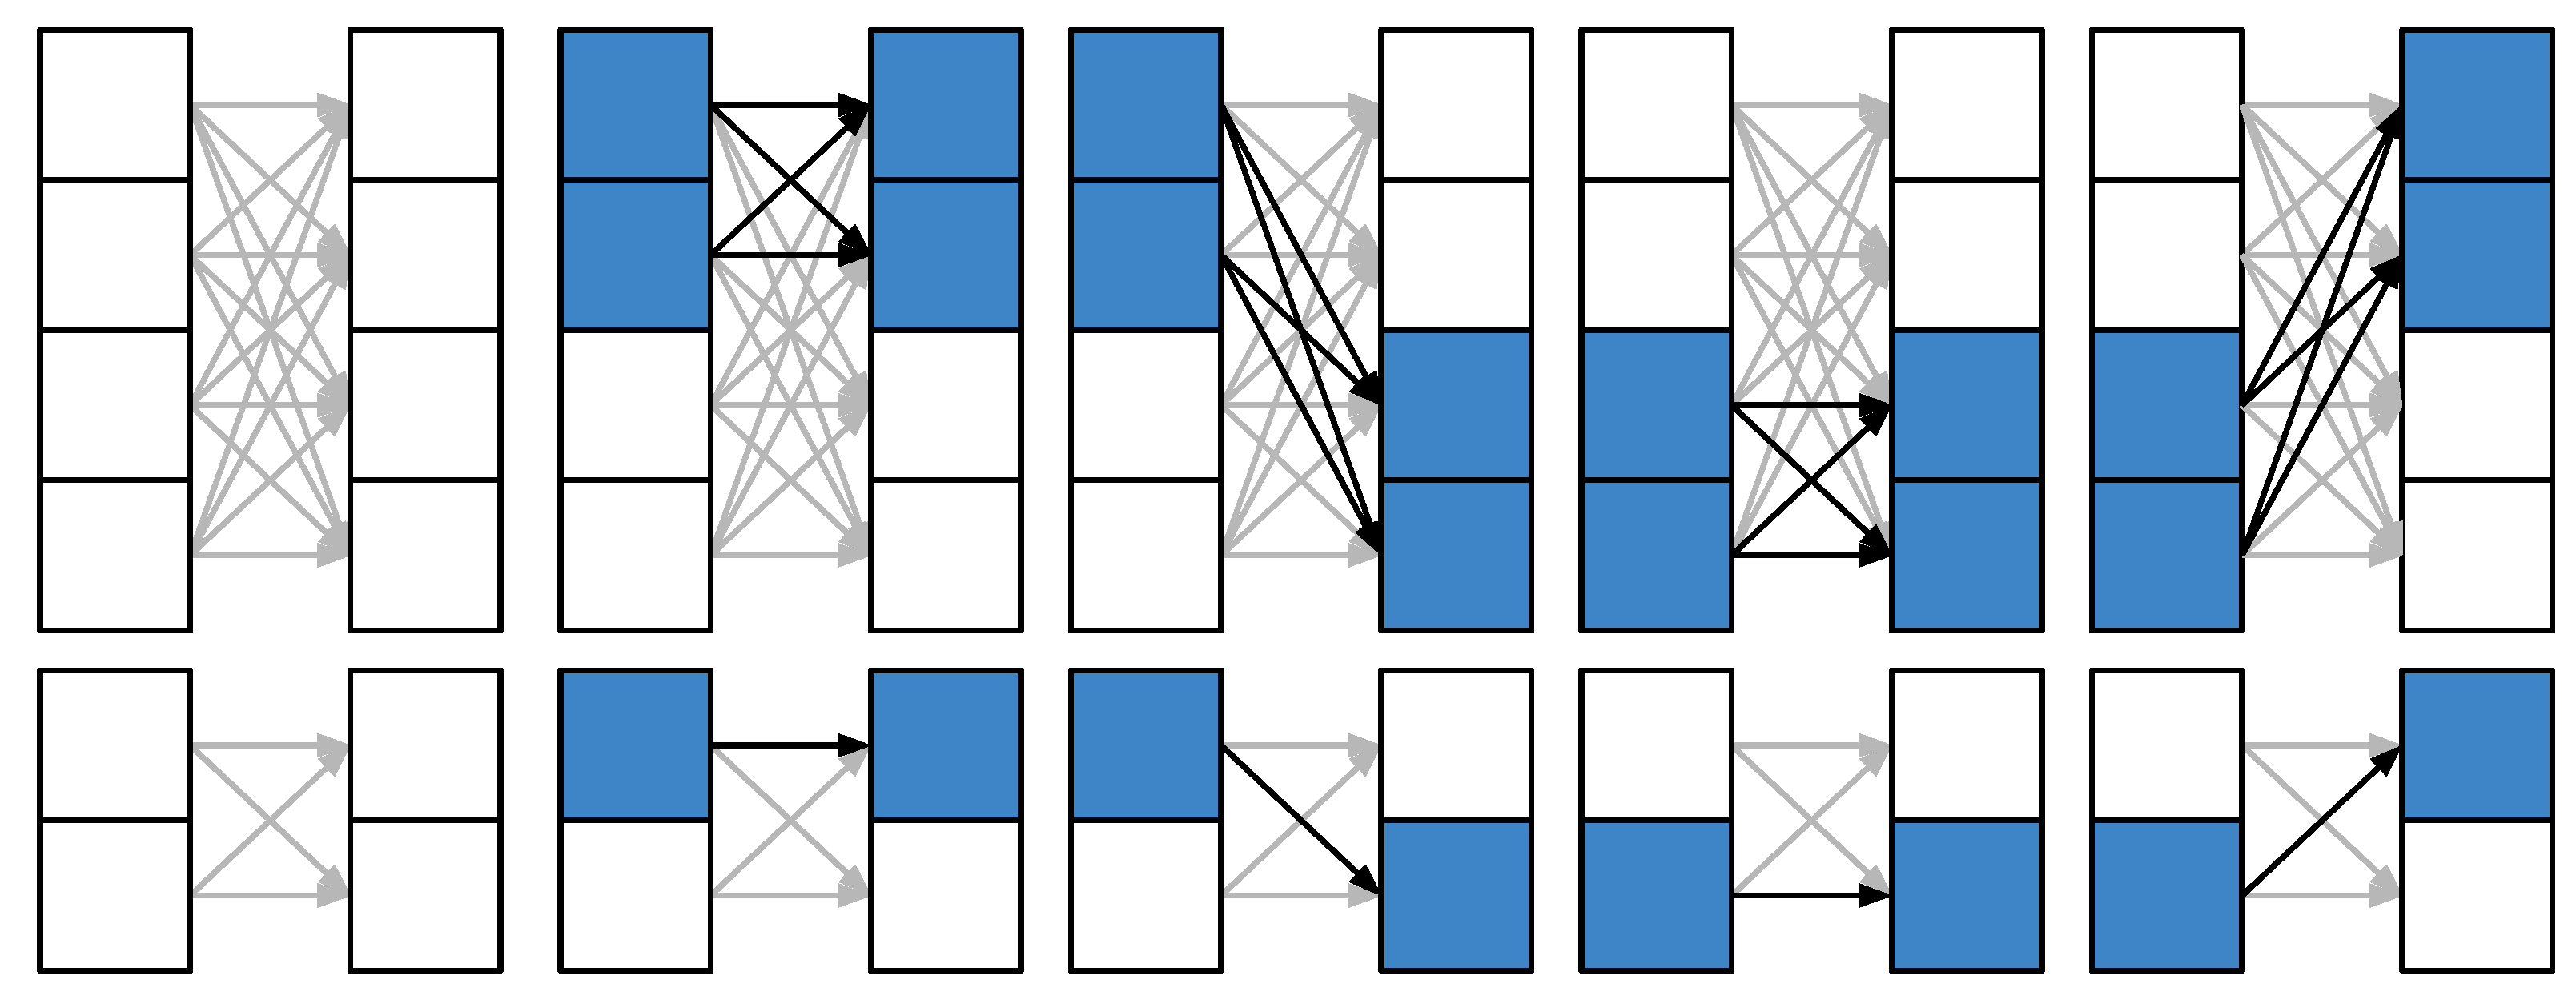
\includegraphics[width=0.8\linewidth]{fig/serialexec}
    \end{center}
    \caption{The recursive computation done by sub--layer primitive.
      Two levels of recursion are shown, each requiring less cache. }
    \label{fig:full-exec}
  \end{figure}

  This primitive is designed to efficiently use higher levels of cache
  when available, by ensuring that the order of {\bf full image
    primitives} are executed in a cache--friendly way.  This is
  achieved in a recursive fashion, where each successive recursive
  step requires half the memory to fit the whole working set inside
  the cache.  Two levels of recursion are shown for the case of
  $\alpha = \beta = 4$ are shown on Fig.~\ref{fig:full-exec}.  In the
  first step (first row in Fig.~\ref{fig:full-exec}), both the number
  of input and output images are divided in half.  The next recursive
  step (second row in Fig.~\ref{fig:full-exec}) is then applied for
  all 4 possible subdivisions.  Note how the second level of recursion
  requires storage for 2 input and 2 output images in order to fit the
  whole working set inside cache, while the first level requires twice
  as much.  The order in which the 4 recursive problems are solved
  further increases cache reuse.  In the case when $\alpha \ge 2\beta$
  or $\beta \ge 2\alpha$ a simpler recursive step is performed, by
  dividing only the input/output images in half and solving two
  recursive sub--problems.

  {\bf Full layer primitive} divides the computation of $B$ sets of
  $\alpha' S$ output images into sets of sub--layer primitives.  Each
  of $T$ available threads is given an ordered list of primitives to
  execute.

  The main goal of the primitive is to equally divide the work among
  the $T$ threads such that once invoked they all finish roughly at
  the same time.  As described above, the $B$ sets of $\alpha'S$
  output images of size $N_x' \times N_y' \times N_z'$ can regarded as
  a $5D$ tensor of size $B \times (\alpha'S) \times N_x \times N_y
  \times N_z$.  We take a recursive approach to our static scheduling
  algorithm.  The input to our algorithm is a set of $T$ threads, and
  a $5D$ tensor of values that has to be computed.

  For the base case of our algorithm, when $T=1$, a sub--layer
  primitive that computes the values of the $5D$ tensor is {\bf
    appended} to the list of primitives to be executed by the given
  thread.

  Our algorithm has two different recursive steps.  The first version
  of the recursive step first finds the smallest prime $p$ that
  divides $T$.  It then divides the set of $T$ threads into $p$ sets
  of $T/p$ threads, and the $5D$ tensor into $p$ equal sub--tensors by
  slicing it along the highest significant dimension that has a size
  of at least $p$.  It then recursively solves the $p$ sub--problems
  for each set of $T/p$ threads and each equally sized sub--tensor.
  If no dimension of the tensor is larger or equal than $p$, we apply
  the base case on an arbitrary available thread.  If the dimension of
  the tensor along which the splicing was performed is not divisible
  by $p$, another recursive problem is solved for all $T$ threads and
  the remaining sub--tensor.  Note that the size of the sub--tensor of
  each recursive sub--problem has at least $p$ times less elements.

  The assigned lists of primitives to be executed by each thread will
  be exponentially smaller in size, with possibly some threads
  executing an extra, computationally cheap primitives.  Thus, we
  expect the threads to be done roughly at the same time.

  As our previous primitives assume computation of multiple of $S$
  images, splicing along the second most significant dimension (of
  size $\alpha'S$) is done only when $\alpha' \ge p$.

  Note that in the last recursive call for the remainder of the
  sub--divided tensor, the value of $T$ doesn't decrease.  The depth
  of recursion can reach up to $\log_2 E$, where $E$ is the number of
  elements in the $5D$ tensor, which can be very large.  As the
  scheduling is done during compile--time, this can significantly
  increase the compile time, and create ``code bloat''.

  To prevent this we introduce the second version of the recursive
  step, which is applied when the number of elements of the $5D$
  tensor is very small (compared to the original tensor).  In this
  case we divide the tensor along the most significant dimension
  larger than $T$ into $T$ sub--tensors, some of which are larger than
  others, after which $T$ base cases are applied and the work is
  scheduled on the $T$ threads.  The basic idea is that once
  computation required for the sub--tensor is small compared
  ($\epsilon$ times smaller) to the overall computation required for
  the whole layer, we can allow for some cores to do a bit more work
  than others without hurting overall performances.  In our
  implementation we chose $\epsilon = 0.008$.  This limits the
  recursion to maximal depth of $7$ while not allowing any single core
  to perform more then $1\%$ more work than other cores.

  \begin{figure}
    \begin{center}
      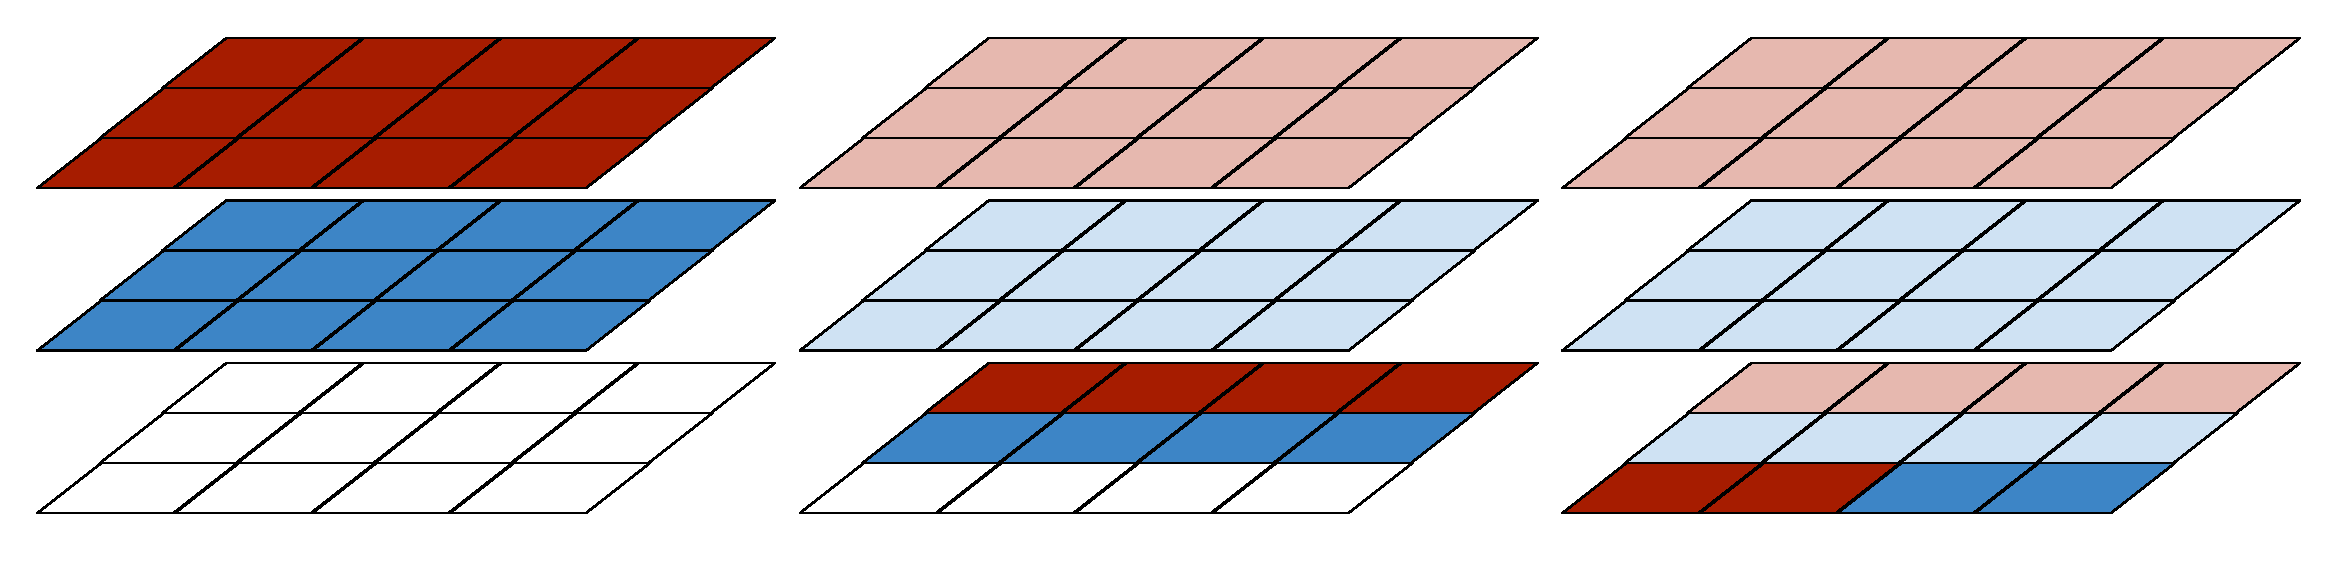
\includegraphics[width=0.67\linewidth]{fig/static2}
    \end{center}
    \caption{Computing the values of $F'=3$ channels of 2D images of
      size $4 \times 3$ using $T=2$ threads.  The three columns
      represent three stages.  The dark blue/red represent the values
      scheduled to be computed by $1^{st}/2^{nd}$ core.}
    \label{fig:problem-subdivision}
  \end{figure}

  An example of such scheduling for the special case of $B=1$, $F'=3$
  and $S=1$ and 2D images of size $4 \times 3$ is shown on
  Fig.~\ref{fig:problem-subdivision}.

  There are multiple benefits of our approach.  First, note that all
  the cores perform exactly the same computation.  When using multiple
  virtual threads per physical core, each thread can benefit from $L1$
  instruction cache.  Additionally, when multiple threads compute
  different images of the layer (as in the first step in
  Fig.~\ref{fig:problem-subdivision}), they access the elements of the
  input images in the exact same order.  This will yield high hit rate
  of the higher levels of cache shared between cores.

  \subsection{Input image padding and strided convolution}

  As mentioned before, in order to be usable for the backward pass,
  our primitive has to support either implicit or explicit zero
  padding of input images.  When the input images are large, and
  kernels small, explicit zero padding of the input image only
  slightly increases the computational cost.  However, as the images
  get smaller this overhead can become significant.

  We support implicit padding along an arbitrary of dimensions by
  modifying the lines 8--11 of
  Algorithm~\ref{alg:serial-forward-subtask}.  Instead of looping over
  all possible kernel offsets, for each invocation of the primitive,
  we provide additional run--time parameters, a pre--computed limits,
  for which the kernels offset are valid.

  Additionally, once might consider a hybrid approach, where along
  some directions the input is explicitly padded, while along the
  other we perform implicit computation.

  Our algorithm can easily be modified to support strided
  convolution/cross--correlation, which is supported in our
  implementation.  This is accomplished by simply modifying the line
  $18$ of Algorithm~\ref{alg:serial-forward-subtask} to account for
  the strides.
